\chapter{Selecci\'on de caracteres}
\section*{Introducci\'on}
\index{Caracter!Homolog\'ia}
\index{Caracter!Definici\'on}

En un an\'alisis filogen\'etico clad\'istico es necesario identificar y usar caracteres hom\'ologos, de hecho, la importancia de los caracteres es tal que Hennig (1968) se refer\'ia a los espec\'imenes estudiados como semaforontes (\textbf{o los que llevan caracteres}). A\'un a pesar del papel central del concepto de car\'acter, la definici\'on no es tan f\'acil.


Richards se\~nala que el t\'ermino 
\textbf{car\'acter} no est\'a bien definido (Richards, 2003) y que su 
reconocimiento depende en gran parte del entrenamiento del tax\'onomo 
(Richards, 2002). 
Es por eso que la mayor\'ia de las ocasiones se 
enfatiza en la importancia de un \textbf{an\'alisis de caracteres} 
profundo y concienzudo (v.g., Hennig, 1968; Neff, 1986; Rieppel \& 
Kearny, 2001)\footnote{Este an\'alisis de caracteres tambi\'en implica revisar las afirmaciones cuatitativas o cualitativas hechas, ver 
Wiens 2001 
% Syst Biol (2001) 
% Character Analysis in Morphological Phylogenetics: Problems and Solutions
% 50 (5): 689-699.doi: 10.1080/106351501753328811
}.
\index{Caracter!Codificaci\'on} 

Las ideas de car\'acter y homolog\'ia usadas aqu\'i 
son independientes del tipo de caracteres usados, pero es mucho m\'as 
sencillo presentar la discusi\'on en t\'erminos de caracteres 
morfol\'ogicos. M\'as adelante se tratar\'a directamente el tema de los 
caracteres moleculares. 

Aunque no existe una f\'ormula m\'agica para reconocer caracteres hom\'ologos, 
la principal idea es la similitud ''especial'', basada en 
la definici\'on de homolog\'ia como \textbf {similar por ancestr\'ia 
com\'un} (Rieppel \& Kearny, 2001; \textit {contra} Kluge 2002, 
Grant \& Kluge, 2004). Por similitud no debe entenderse solo el 
parecido general, sino que existe una correlaci\'on estructural y de 
posici\'on (la similitud y conjunci\'on en el sentido de Patterson, 
1981) del car\'acter en los taxa comparados.\index{Caracter!Test 
de Patterson} 

Por ejemplo, los brazos humanos, las alas de los murci\'elagos y las 
patas de los caballos presentan una estructura \'osea muy similar, 
con diversos huesos colocados en las mismas posiciones, y en general 
el miembro completo est\'a en la misma posici\'on con respecto al 
cuerpo en los tres taxa, aunque sus formas son muy diferentes. 


Otro factor importante a tener en cuenta son los ''grados'' o 
niveles de generalidad de homolog\'ia. Es decir, que una estructura 
es hom\'ologa con otra en un cierto grado, pero no comparable con 
ella en otro. Por ejemplo, artr\'opodos y vertebrados comparten la 
cefalizaci\'on y el tener miembros pareados. Comparar directamente 
esas estructuras no es apropiado, aunque es posible que sean 
hom\'ologas a nivel molecular, donde los mismos genes controlan el 
desarrollo de estas estructuras, pero la larga historia 
independiente de cada linaje hace imposible una comparaci\'on de las 
estructuras como homolog\'ias, aunque no prohibe una comparaci\'on 
funcional. 

Es importante recalcar que cuando alguien compara los 
caracteres de diferentes taxa, hace una inferencia fuerte sobre los 
caracteres: se trata del mismo car\'acter en los taxa; es decir, da 
una identidad hist\'orica al car\'acter al hacerlo el mismo car\'acter 
por homolog\'ia, aunque est\'en modificados los distintos 
estados (Hennig, 1968; Kluge, 2002). Esto es lo que le da soporte al 
uso de la congruencia de caracteres para descubrir las sinapomorf\'
ias que le dan identidad hist\'orica a los grupos supraespec\'ificos.

 
La selecci\'on y observaci\'on de caracteres, no solo morfol\'ogicos, es un trabajo que s\'olo se aprende mediante el trabajo continuo con los datos derivados de los espec\'imenes en el laboratorio y con una lectura cr\'itica de la literatura sobre el grupo. Es importante que usted pueda reconocer cu\'ando los caracteres usados en una descripci\'on, una clave o un an\'alisis filogen\'etico cumplen o no con el requisito de la identidad hist\'orica.


Algunos libros de texto  sistem\'atica, presentan distintos criterios de reconocimiento de caracteres (por ejemplo Hennig, 1968; Wiley \&  Lieberman 2011), aunque no es posible plantear reglas estrictas o situaciones de casos perfectos, eso no es un motivo para suponer que los caracteres morfol\'ogicos carecen de base conceptual y por ello deben ser excluidos del an\'alisis (\textit{contra} Scotland et al., 2003).

Existen algunos criterios b\'asicos aplicables en general a los caracteres: para cada car\'acter se reconocen diversos estados alternativos de ese car\'acter, los cuales son llamados estados de car\'acter o simplemente estados. Es posible que un car\'acter no sea aplicable a todos los organismos de estudio, pero dentro de los organismos donde es aplicable, los estados de un car\'acter deben dividir el universo en al menos dos grupos mutuamente excluyentes, cada uno de ellos reconocible por un estado de caracter.


Dado que se tratan los caracteres como identidades hist\'oricas, se debe ser cuidadoso con \textbf{NO} crear estados de car\'acter que sirvan como ''cajas de basura''. Por ejemplo, en el car\'acter ''color: (a) rojo; (b) otro color'', el estado (b) es ambiguo y puede contener individuos de diferentes colores, cuya \'unica (falsa) similitud sea que no poseen el color rojo, pero no existe una identidad hist\'orica defendible, es decir el NO color rojo se ha generado desde m\'ultiples ancestros.


Todos los estados del car\'acter deben representar una unidad hist\'orica, independientemente de si el estado es el apom\'orfico o el 
plesiom\'orfico. 
Siempre que encuentre un car\'acter donde uno de los estados est\'a definido como negaci\'on (incluidas las ausencias), 
debe revisar cuidadosamente que el estado ''negativo'' indique claramente una unidad.


Cuando los caracteres solo tienen dos estados, no es necesaria ninguna suposici\'on sobre la ''direcci\'on del cambio''; 
sin embargo, cuando hay m\'as de dos estados, la direcci\'on es una pregunta importante. 
Algunos caracteres simplemente no dan posibilidad de escoger una direcci\'on particular (por ejemplo, las bases nucleot\'idicas), 
por lo cual son caracteres no ordenados. 
Bajo una posici\'on,  uno puede asignar un posible orden a los caracteres que se leen como diversos grados de homolog\'ia, 
sin asumir nada sobre el proceso evolutivo, 
por ejemplo, el caracter: 


\begin{small}
Pilosidad en la pata: 
\begin{enumerate}[start=0]
\item solo en el extremo anterior
\item hasta la mitad
\item todal a superficie
\item toda la pata y con presencia de pelos m\'as largos en el extremo posterior
\end{enumerate}	
\end{small}


podr\'ia ordenarse desde 0 hasta 3 (hacerlo aditivo) para reflejar que existe un mayor grado de homolog\'ia entre, por ejemplo, el estado 2 y 3, que 1 y 3. 
La otra posici\'on no privilegiar\'a ning\'un cambio con respecto a otro y la direcci\'on se asignar\'ia por la congruencia con otros caracteres (el car\'acter es no aditivo).


En otros casos, la identidad hist\'orica es dif\'icil de apreciar; por ejemplo, ''transparentable con KOH: (a) s\'i, (b) no'', suponiendo que el estado (b) no es problem\'atico, el car\'acter como un todo parece ser m\'as un artefacto de laboratorio que una propiedad heredable del organismo. En esa misma l\'inea est\'an caracteres como ''n\'umero de componentes en PCA: (a) uno; (b) dos''.


Al tratarse los estados de caracter como alternativas, un mismo organismo no puede poseer dos estados o m\'as estados del mismo car\'acter: para nuestra visi\'on de homolog\'ia de las alas y los miembros anteriores, no pueden existir \'angeles o centauros, con dos versiones diferentes del miembro anterior en el mismo organismo. Este es el criterio de ''conjunci\'on'' de Patterson. sin embargo, hay que tener en cuenta que existen homolog\'ias seriadas que \textbf{contradicen} esta idea, no solo en organismos segmentados como an\'elidos y artr\'opodos, sino en otros donde la segmentaci\'on no es clara (e.g., hojas de las plantas, pelos de los mam\'iferos, etc.). El criterio de conjunci\'on de Patterson es un llamado al reconocimiento de las estructuras que se usan como caracteres en el an\'alisis filogen\'etico.

%\section{Materiales}

\section*{T\'ecnicas}


Use el dibujo al final de la pr\'actica el c\'ual corresponde a la figura 1 en Sokal (1983). 
Los ''organismos'' son camin\'aculos, seres hipot\'eticos creados por J. Camin para estudios sobre clasificaciones en fen\'etica.\footnote{Copyright, Society of Systematic Biologists, se reproduce con permiso} A partir de los dibujos:


%\section{M\'etodos}


\begin{enumerate}
	\item Elabore una peque\~na gu\'ia morfol\'ogica de los organismos, de modo que pueda diferenciar las diferentes estructuras en los diferentes organismos (en buen romance significa poner nombres a sus organismos y ligar tales nombres a estructuras f\'acilmente reconocibles; el ejercicio m\'as cercano en un an\'alisis para separar por \textbf{morfos} sus organismos).

	\item Elabore un listado de los diferentes caracteres de los organismos, reconozca al menos 5 caracteres \'unicos y 5 compartidos. Anote en una hoja separada los organismos y sus estados.
	
	\item Intercambie su listado (acompa\~nado de la gu\'ia morfol\'ogica y los nombres de los organismos) con un compa\~nero: 
	
	\begin{enumerate}
		\item Trate de reconocer los caracteres que su compa\~nero describi\'o, y anote c\'uales organismos poseen esos caracteres.
		\item En caso de ser necesario, re-escriba los caracteres de su compa\~nero e indique la raz\'on de sus cambios.
	\end{enumerate}
	
	\item Compare la lista de caracteres por organismos que usted 
	realiz\'o con la que su compa\~nero re-escribio.

\end{enumerate}


\pregunta{


\begin{enumerate}
	\item Haga un ejercicio cr\'itico de los caracteres de sus compa\~neros:
	 
	\begin{enumerate}
		\item ?`est\'an bien definidos?	
		\item ?`hay impl\'icita una transformaci\'on?
		\item ?`usaron de la misma forma la similaridad?
	\end{enumerate}

	\item Trate de localizar los motivos de sus aciertos y fallas cuando trabaj\'o con los caracteres de su compa\~nero. ?`Son esos motivos consistentes con la cr\'itica a los caracteres?

	\item Eval\'ue la cr\'itica de su compa\'nero a sus caracteres: ?`es posible reescribir los caracteres para mejorarlos? Si as\'i lo cree, reescr\'ibalos; en caso contrario, d\'e argumentos para desechar el car\'acter o para mantener su definici\'on actual.
\end{enumerate}
}


\preguntaGral{

\begin{enumerate}
	\item Use la literatura de la que disponga sobre un grupo en particular, trate de evaluar los caracteres presentes y h\'agase preguntas similares a las que realiz\'o cuando examin\'o los caracteres de sus compa\~neros.\\

	\item Si es posible, trate de usar y contrastar un an\'alisis filogen\'etico con una descripci\'on tradicional del mismo grupo.\\

	\item Pleijel (1995) argument\'o que los \'unicos caracteres v\'alidos son las presencias, por lo que todos los caracteres son una enumeraci\'on  de presencia/ausencia (no hay \textbf{estados de car\'acter}), trate de identificar las posibles ventajas y falencias de esa aproximaci\'on.\\

	\item Lea el art\'iculo de Goloboff et al., 2006 e identifique la forma como se manejan los caracteres cuantitat\'ivos. ?`usan un esquema similar al usado para los caracteres discretos?
\end{enumerate}

}

%\newpage
\section*{Literatura recomendada}

%
% revisar el esquema de citacion en esta sección
%

de Pinna (1991) [Ofrece una visi\'on a la formulaci\'on de los caracteres].

Kluge, 2003 [Una cr\'itica al uso de la \textbf{similitud} como criterio de selecci\'on de caracteres].

Neff, 1986 [Una normalizaci\'on del an\'alisis de caracteres].

Patterson, 1982 [La \textbf{verdadera prueba de homolog\'ia}].

Platnick, 1979 [Un art\'iculo cl\'asico sobre la jerarqu\'ia -cladismo de patr\'on-, tanto de caracteres como de taxa].

Pleijel, 1995 [Una visi\'on al manejo de caracteres, diferente a la ofrecida aqu\'i].

Rieppel \& Kearny, 2002 [Una visi\'on cr\'itica y extensa de la selecci\'on de caracteres, con ejemplos emp\'iricos].

\begin{figure}
\centering
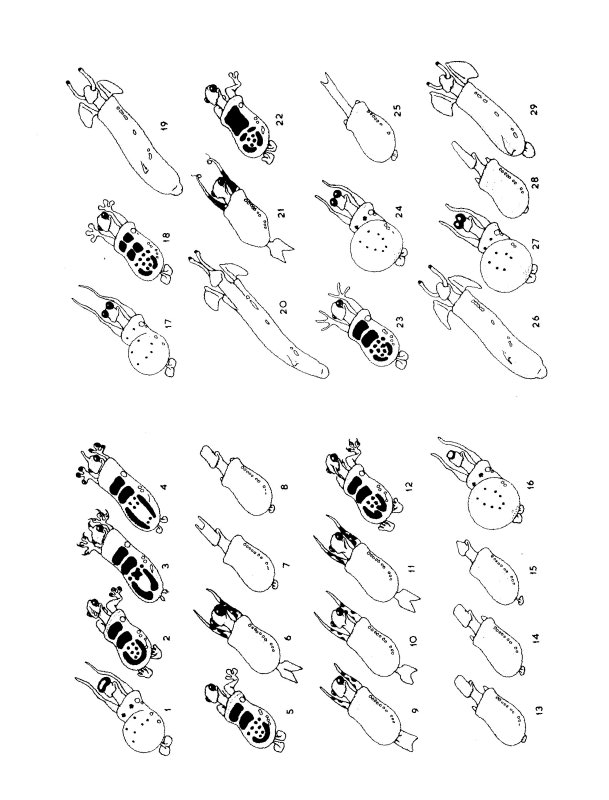
\includegraphics[scale=0.75]{./practica01/cami0.jpg}
% \resizebox{7in}{7in}{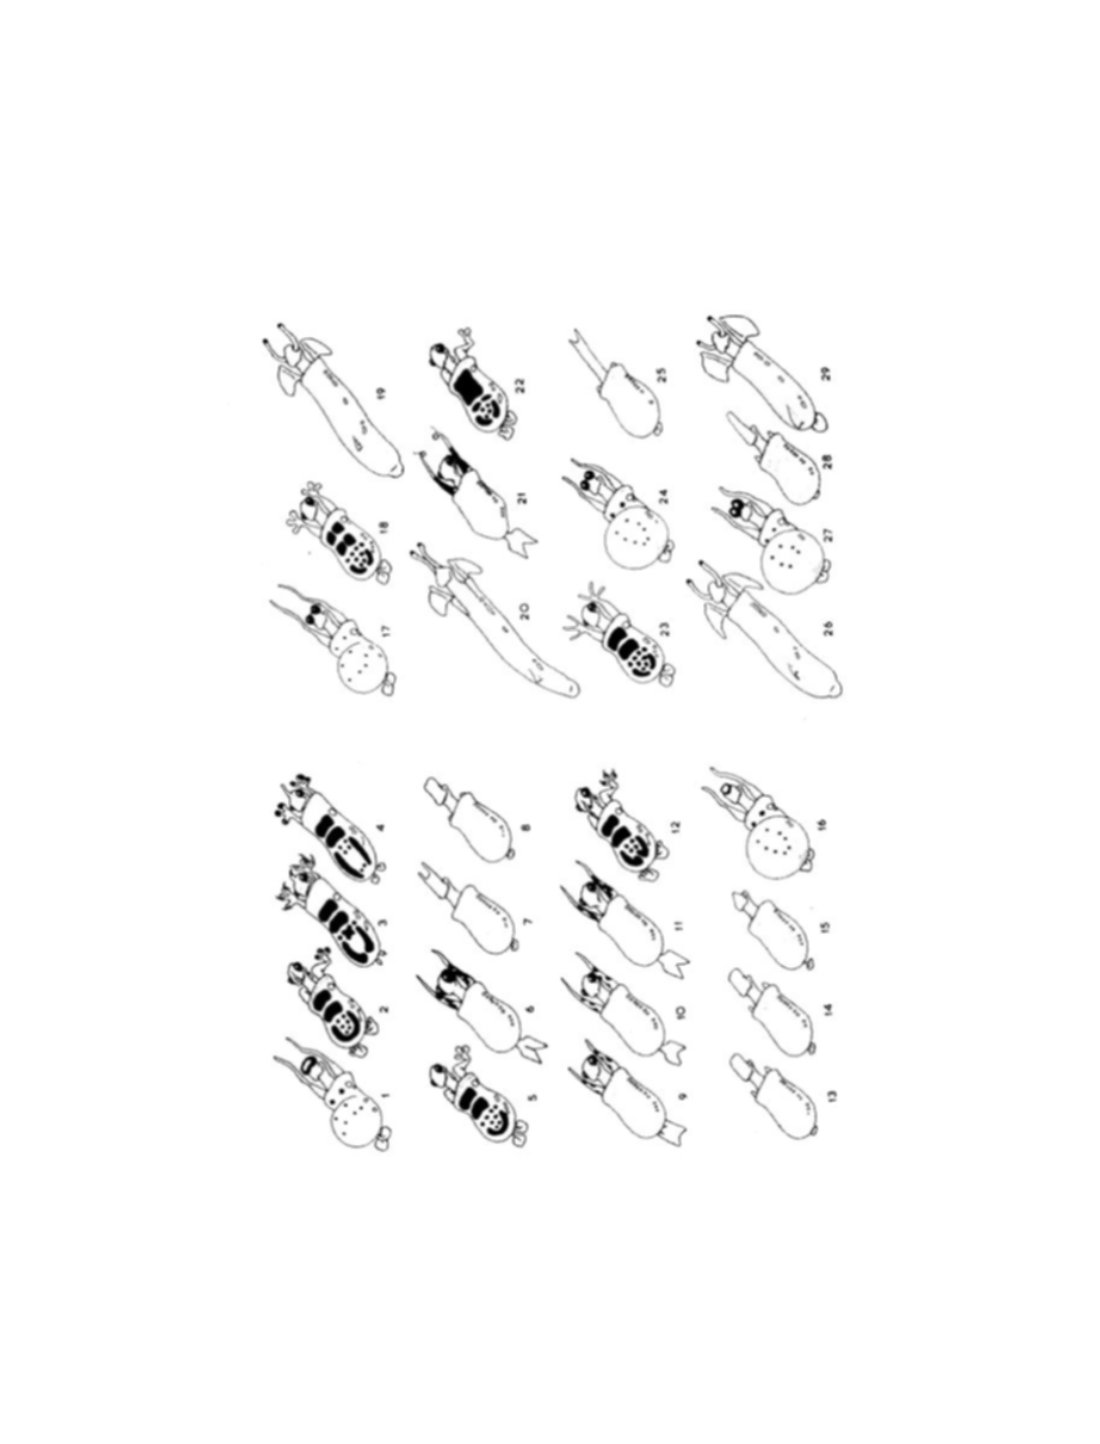
\includegraphics[]{camin.jpg}}
% \scalebox{0.80}[0.40]{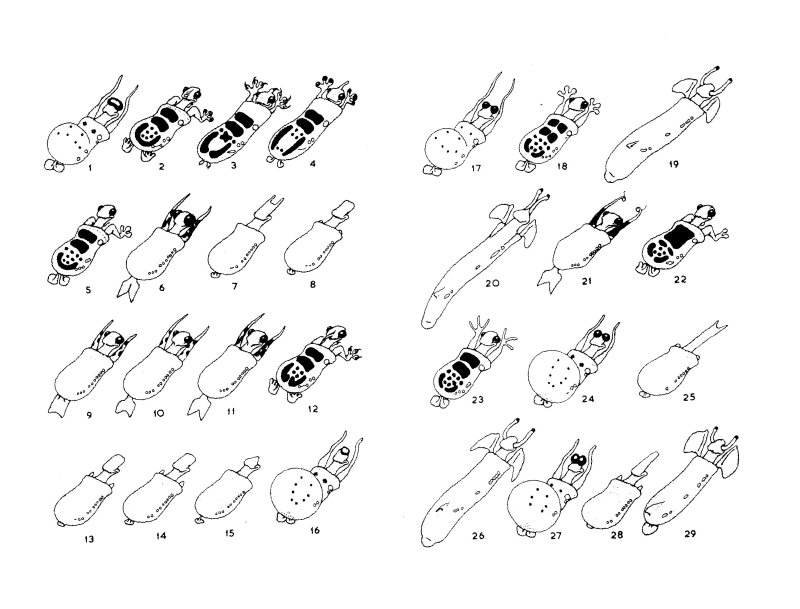
\includegraphics[clip,scale=1]{cami.jpg}}
% \resizebox{5in}{9in}{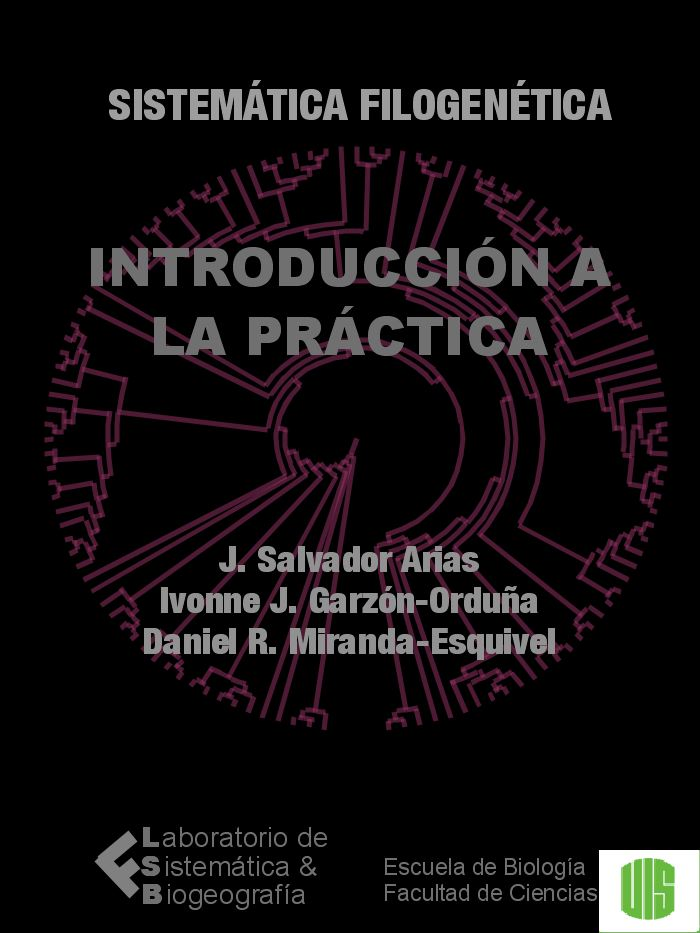
\includegraphics[clip,scale=1]{2_p.jpg}}
% \includegraphics[bb= 600 920 100 0, scale=0.30]{portada.jpg}
% 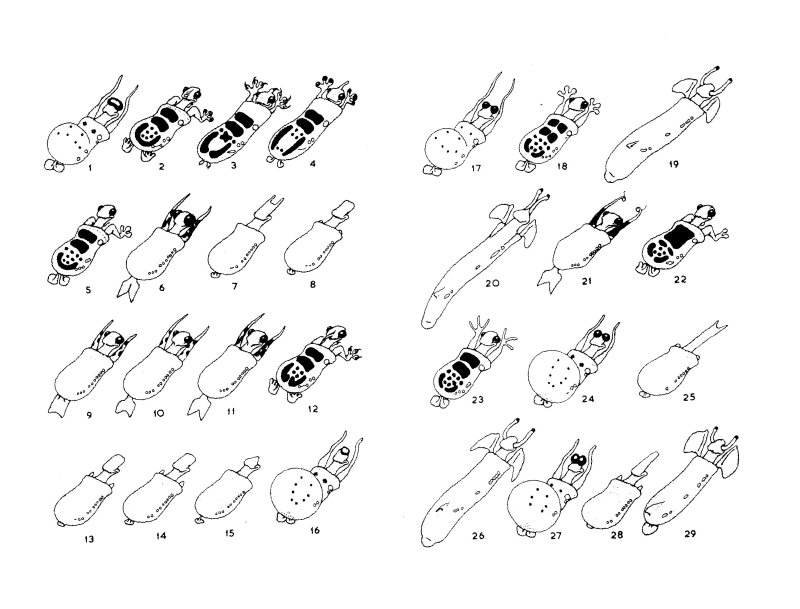
\includegraphics[bb= 100 200 100 0,scale=1]{cami.jpg}
% ,scale=0.5
\caption{Los Camin\'aculos, tomado de Sokal (1983) \\Copyright \textit{Society of Systematic Biologists}, se reproduce con permiso.}
% \vspace{-2mm}
\end{figure}

